% 2010 年广东卷文科第 9 题：多面体 ABC-A'B'C'。
% 来源 PDF：普通高考/2010/2010广东文.pdf，SHA-256 dd04b2053a22c854a9abe1ee03241fc04d5a25c91cda1d7997183bdfaa4a8c6f。
% 原页：第 1 页（A3 三栏）第 1 栏下部，书页码 595。
% 重绘依据：ABC 为正三角形；AA'、BB'、CC' 平行且 CC'⊥平面 ABC；
%   3AA'=(3/2)BB'=CC'=AB。AC 与 CC' 为不可见棱，画虚线。
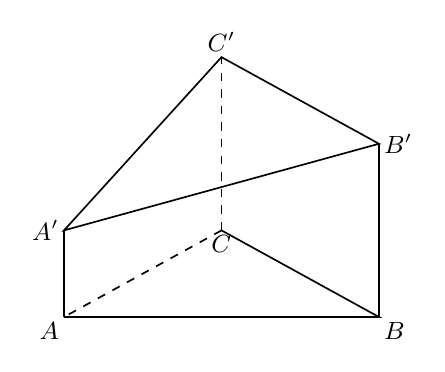
\begin{tikzpicture}[semithick, every node/.style={inner sep=1.6pt, font=\small}]
  \coordinate (A) at (0,0);
  \coordinate (B) at (4,0);
  \coordinate (C) at (2,1.1);
  \coordinate (Ap) at (0,1.1);
  \coordinate (Bp) at (4,2.2);
  \coordinate (Cp) at (2,3.3);

  \draw (A) -- (B) -- (C);
  \draw[dashed] (C) -- (A);
  \draw (A) -- (Ap);
  \draw (B) -- (Bp);
  \draw[dashed] (C) -- (Cp);
  \draw (Ap) -- (Bp) -- (Cp) -- cycle;

  \node[below left] at (A) {$A$};
  \node[below right] at (B) {$B$};
  \node[below] at (C) {$C$};
  \node[left] at (Ap) {$A'$};
  \node[right] at (Bp) {$B'$};
  \node[above] at (Cp) {$C'$};
\end{tikzpicture}
